\section{Architecture}
For building up a network architecture two methods is broadly used in games Peer-to-Peer and Client-server based architecture. 

%http://gafferongames.com/networking-for-game-programmers/what-every-programmer-needs-to-know-about-game-networking/

\subsection{Client-Server}
The Client-Server model consist of clients and a server as shown in Figure \ref{fig:server_client}. 

\begin{figure}[H]
\centering
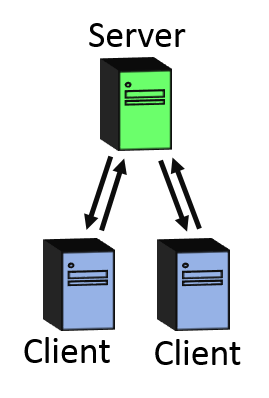
\includegraphics[scale=1]{figures/network/server_client}
\label{fig:server_client}
\caption{An illustration of the server/client model.}
\end{figure}

In the traditional client server model, the server is where all the computation happens and is communicated out to the client.
Whereas the clients are essentially \textit{dumb terminals} which is computers that purely redirect the input from the user of the client to the server. 
The server then computes what should happen and then send that information back to the clients, that then updates their games state accordingly.

\subsection{Peer-to-Peer}
The Peer-to-peer model consists purely of peers with no dedicated server.
This means peers can communicate directly with other peers as shown in Figure \ref{fig:peer_peer}

\begin{figure}[H]
\centering
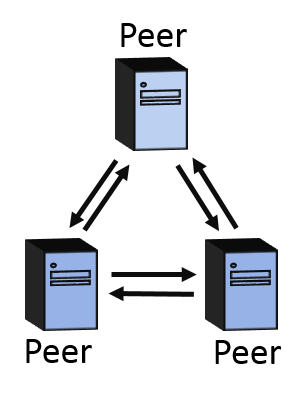
\includegraphics[scale=1]{figures/network/peer_peer}
\label{fig:peer_peer}
\caption{An illustration of the Peer-to-peer model.}
\end{figure}

Peer-to-Peer (\textit{P2P}) network model in games ideally consists of turns.
Each turn the players gathers the different input from each player who then individually executes all the commands on each machine.
The purpose of this is that, given a deterministic game, the game that are running on each individual computer will be running the exact same code. 
Therefore given the game is deterministic the game state will be exactly the same on each computer. 
%http://www.gamasutra.com/view/feature/131503/1500_archers_on_a_288_network_.php

\subsection{Choosing an architecture}
The client-server architecture is popular in games because it does not limit the update rate of the game based on the connection of the slowest player, but instead only based on the connection of the server.
Thus we choose the client-server architecture.